\chapter{flipper 2000}
\lhead[tempest 2000]{}
\label{sec:listing}
\lstset{style=68KStyle}

The data structure as given in the source code is:

\begin{lstlisting}
s_flipper: 
  dc.l 4        ; 4 faces in this object, a shaded solid Flipper
    
	dc.w $f0       ; Face colour - Red.
	dc.w 3,$8000   ; vertex index, intensity.
	dc.w 1,$c000   ; vertex index, intensity.
	dc.w 0,$ff00   ; vertex index, intensity.
	dc.w 0
    
	dc.w $f4       ; Face colour - Orange.
	dc.w 4,$4000   ; vertex index, intensity.
	dc.w 2,$8000   ; vertex index, intensity.
	dc.w 0,$c000   ; vertex index, intensity.
	dc.w 0
    
	dc.w $f4       ; Face colour - Red.
	dc.w 5,$8000   ; vertex index, intensity.
	dc.w 1,$c000   ; vertex index, intensity.
	dc.w 0,$ff00   ; vertex index, intensity.
	dc.w 0
    
	dc.w $f0       ; Face colour - Orange.
	dc.w 6,$4000   ; vertex index, intensity.
	dc.w 2,$8000   ; vertex index, intensity.
	dc.w 0,$c000   ; vertex index, intensity.
	dc.w 0

fverts: dc.w 9,9,5,9,13,9,1,0,17,0,1,18,17,18
\end{lstlisting}

A little more explanation, taking the first entry in the structure:
\begin{lstlisting}
	dc.w $f0		  ; Face colour - Red.
	dc.w 3,$8000	; Index into fverts, followed by intensity value.
	dc.w 1,$c000	; Index into fverts, followed by intensity value.
	dc.w 0,$ff00	; Index into fverts, followed by intensity value.
	dc.w 0        ; Padding that rounds up the entry to 16 bytes
\end{lstlisting}

We can see that the middle three entries start with an index into the array \icode{fverts} we listed above.
The index is pair-wise, so for example an index of \icode{3} must be multiplied by 2, and then counting into \icode{fverts}
starting from 0 we end up at the 7th element and the pair: \icode{1,0}. We can make this more explicit by breaking out the
presentation of \icode{fverts} to match the way it's used:
\begin{lstlisting}
fverts: dc.w 9,9   ; Index 0
        dc.w 5,9   ; Index 1
        dc.w 13,9  ; Index 2
        dc.w 1,0   ; Index 3
        dc.w 17,0  ; Index 4
        dc.w 1,18  ; Index 5
        dc.w 17,18 ; Index 6
\end{lstlisting}

What are these pairs of numbers? They are (x,y) co-ordinates of course. It turns out \icode{vertex} is just a fancy term
for a point in two-dimensional space. So we can now begin to discern what this data structure is: it contains 4 sets of
3 vertices each. If you have 3 points in space, you have a triangle. So what we have here is a description of 4 triangles
and each triangle is beign referred to as a 'face'.

Let's use the indices in the first entry to see what the first face gives us. We already saw how to get from an index of
\icode{3} to a vertex of \icode{1,0} above. When we do the other two the three pairs of co-ordinates turn out as:
to be as follows:
\begin{figure}[H]
  {
    \setlength{\tabcolsep}{3.0pt}
    \setlength\cmidrulewidth{\heavyrulewidth} % Make cmidrule = 
    \begin{adjustbox}{width=4cm,center}
      \begin{tabular}{llll}
        \toprule
        Index & X & Y & Description\\
        \midrule
        \icode{3} & \icode{1} & \icode{0} & First vertex.\\
        \icode{1} & \icode{5} & \icode{9} & Second Vertex. \\
        \icode{0} & \icode{9} & \icode{9} & Third Vertex. \\
        \bottomrule
      \end{tabular}
    \end{adjustbox}
  }
\end{figure}

With these, and our specified colour of red (\icode{\$f0}), we can make a triangle:

\begin{figure}[H]
  \centering
  \begin{adjustbox}{width=13cm,center}
    \begin{minipage}[c]{0.48\linewidth}
      \begin{figure}[H]
        \centering
        \begin{adjustbox}{width=5.5cm,center}
          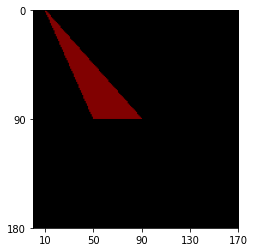
\includegraphics[width=12cm]{src/flipper/flipper_face_1.png}%
        \end{adjustbox}
      \end{figure}
    \end{minipage}
    \begin{minipage}[c]{0.48\linewidth}
      \begin{lstlisting}[basicstyle=\scriptsize\ttfamily]
      dc.w $f0       ; Colour - Red.
      dc.w 3,$8000   ; index, intensity.
      dc.w 1,$c000   ; index, intensity.
      dc.w 0,$ff00   ; index, intensity.
      dc.w 0
      \end{lstlisting}
      \begin{lstlisting}[basicstyle=\scriptsize\ttfamily]
      dc.w 9,9   ; Index 0
      dc.w 5,9   ; Index 1
      dc.w 1,0   ; Index 3
      \end{lstlisting}
      \vspace*{\fill}
    \end{minipage}
  \end{adjustbox}
  \caption{Our three vertices joined together in a triangle. Notice that we\'ve scaled up our co-ordinates by 10. So \icode{(9,9)}, for example, is given as \icode{(90,90)}.}
\end{figure}

One triangle is all very nice, but we have a flipper to build. Should we try a second triangle? Let's see how that goes.

The instructions for our new triangle are in the second paragraph of the \icode{s\_flipper} data structure:
\begin{lstlisting}
	dc.w $f4       ; Face colour - Orange.
	dc.w 4,$4000   ; vertex index, intensity.
	dc.w 2,$8000   ; vertex index, intensity.
	dc.w 0,$c000   ; vertex index, intensity.
	dc.w 0
\end{lstlisting}

When we translate this to co-ordinates from \icode{fverts} we get:
\begin{figure}[H]
  {
    \setlength{\tabcolsep}{3.0pt}
    \setlength\cmidrulewidth{\heavyrulewidth} % Make cmidrule = 
    \begin{adjustbox}{width=4cm,center}
      \begin{tabular}{llll}
        \toprule
        Index & X & Y & Description\\
        \midrule
        \icode{4} & \icode{17} & \icode{0} & First vertex.\\
        \icode{2} & \icode{13} & \icode{9} & Second Vertex. \\
        \icode{0} & \icode{9} & \icode{9} & Third Vertex. \\
        \bottomrule
      \end{tabular}
    \end{adjustbox}
  }
\end{figure}

Not wildly different than our previous effort. Putting our vertices for the two faces together in a single
table we get:
\begin{figure}[H]
  {
    \setlength{\tabcolsep}{3.0pt}
    \setlength\cmidrulewidth{\heavyrulewidth} % Make cmidrule = 
    \begin{adjustbox}{width=5cm,center}
      \begin{tabular}{llll}
        \toprule
        Face & Vertex 1 & Vertex 2 & Vertex 3 \\
        \midrule
        \icode{1} & \icode{1,0} & \icode{5,9} & \icode{9,9} \\
        \icode{2} & \icode{17,0} & \icode{13,9} & \icode{9,9} \\
        \bottomrule
      \end{tabular}
    \end{adjustbox}
  }
\end{figure}

Let's see what we get when we add it in:

\begin{figure}[H]
  \centering
  \begin{adjustbox}{width=13cm,center}
    \begin{minipage}[c]{0.48\linewidth}
      \begin{figure}[H]
        \centering
        \begin{adjustbox}{width=5.5cm,center}
          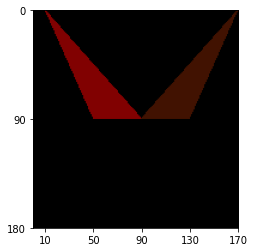
\includegraphics[width=12cm]{src/flipper/flipper_face_2.png}%
        \end{adjustbox}
      \end{figure}
    \end{minipage}
    \begin{minipage}[c]{0.48\linewidth}
      \begin{lstlisting}[basicstyle=\scriptsize\ttfamily]
dc.w $f4       ; Colour - Orange.
dc.w 4,$4000   ; index, intensity.
dc.w 2,$8000   ; index, intensity.
dc.w 0,$c000   ; index, intensity.
dc.w 0
      \end{lstlisting}
      \begin{lstlisting}[basicstyle=\scriptsize\ttfamily]
dc.w 9,9   ; Index 0
dc.w 13,9  ; Index 2
dc.w 17,0  ; Index 4
      \end{lstlisting}
      \vspace*{\fill}
    \end{minipage}
  \end{adjustbox}
  \caption{Adding in our second triangle}
\end{figure}

OK, things are starting to take shape. Here are the vertices for all four faces together:

\begin{figure}[H]
  {
    \setlength{\tabcolsep}{3.0pt}
    \setlength\cmidrulewidth{\heavyrulewidth} % Make cmidrule = 
    \begin{adjustbox}{width=5cm,center}
      \begin{tabular}{llll}
        \toprule
        Face & Vertex 1 & Vertex 2 & Vertex 3 \\
        \midrule
        \icode{1} & \icode{1,0} & \icode{5,9} & \icode{9,9} \\
        \icode{2} & \icode{17,0} & \icode{13,9} & \icode{9,9} \\
        \icode{3} & \icode{1,18} & \icode{5,9} & \icode{9,9} \\
        \icode{4} & \icode{17,18} & \icode{13,9} & \icode{9,9} \\
        \bottomrule
      \end{tabular}
    \end{adjustbox}
  }
\end{figure}

Let's see what it looks like when we add in the third triangle:

\begin{figure}[H]
  \centering
  \begin{adjustbox}{width=13cm,center}
    \begin{minipage}[c]{0.48\linewidth}
      \begin{figure}[H]
        \centering
        \begin{adjustbox}{width=5.5cm,center}
          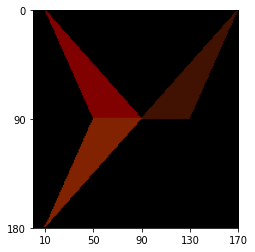
\includegraphics[width=12cm]{src/flipper/flipper_face_3.png}%
        \end{adjustbox}
      \end{figure}
    \end{minipage}
    \begin{minipage}[c]{0.48\linewidth}
      \begin{lstlisting}[basicstyle=\scriptsize\ttfamily]
dc.w $f4       ; Colour - Red.
dc.w 5,$8000   ; index, intensity.
dc.w 1,$c000   ; index, intensity.
dc.w 0,$ff00   ; index, intensity.
dc.w 0
      \end{lstlisting}
      \begin{lstlisting}[basicstyle=\scriptsize\ttfamily]
dc.w 9,9   ; Index 0
dc.w 5,9   ; Index 1
dc.w 1,18  ; Index 5
      \end{lstlisting}
      \vspace*{\fill}
    \end{minipage}
  \end{adjustbox}
  \caption{Adding in our third triangle}
\end{figure}

And the fourth and final triangle:

\begin{figure}[H]
  \centering
  \begin{adjustbox}{width=13cm,center}
    \begin{minipage}[c]{0.48\linewidth}
      \begin{figure}[H]
        \centering
        \begin{adjustbox}{width=5.5cm,center}
          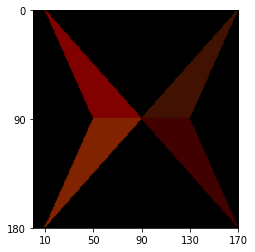
\includegraphics[width=12cm]{src/flipper/flipper_face_4.png}%
        \end{adjustbox}
      \end{figure}
    \end{minipage}
    \begin{minipage}[c]{0.48\linewidth}
      \begin{lstlisting}[basicstyle=\scriptsize\ttfamily]
dc.w $f0       ; Colour - Orange.
dc.w 6,$4000   ; index, intensity.
dc.w 2,$8000   ; index, intensity.
dc.w 0,$c000   ; index, intensity.
dc.w 0
      \end{lstlisting}
      \begin{lstlisting}[basicstyle=\scriptsize\ttfamily]
dc.w 9,9   ; Index 0
dc.w 13,9  ; Index 2
dc.w 17,18 ; Index 6
      \end{lstlisting}
      \vspace*{\fill}
    \end{minipage}
  \end{adjustbox}
  \caption{Adding in our final triangle}
\end{figure}

\begin{lstlisting}
draw_sflipper:
  lea s_flipper,a1
  bra drawsolidxy
\end{lstlisting}

\begin{lstlisting}
drawsolidxy:
  lea in_buf,a0
  move.l a1,(a0)+ ; pointer to our s_flipper data structure
  move.l d2,(a0)+ ; x position to draw flipper
  move.l d3,(a0)+ ; y position to draw flipper
  move.l d1,(a0)+ ; z position to draw flipper
  move.l d4,(a0)+ ; x position of flipper's origin
  move.l d5,(a0)+ ; y position of flipper's origin
  move.l d0,(a0)  ; angle

  move.l #0,gpu_mode
  lea equine,a0
  jsr gpurun      ;do clear screen
  jsr gpuwait
  rts
\end{lstlisting}

